\documentclass[5pt, twocolumn, a4paper, notitlepage, fleqn]{article} % Vertical way
% \documentclass[6pt, landscape, twocolumn, a4paper, notitlepage, fleqn]{article} % Horizontal way
\usepackage{hyperref}
\usepackage[english, activeacute]{babel} %, spanish
\usepackage[utf8]{inputenc}
\usepackage{fancyhdr} % Fancy headers
\usepackage{enumitem} % Enable enumerations
\usepackage{amsbsy, amssymb, amsmath, mathtools} % Enable math symbols
\usepackage{ifthen} % To enable some conditional programming in LaTeX
\usepackage[usenames, dvipsnames]{xcolor} % extra colors
\usepackage{geometry} % A simple way to change the length and layout of different elements
\usepackage{lastpage}  % A simple way to go to the last page xd
\usepackage{listings} % To add code
\usepackage{graphicx, wrapfig} % To add images
\usepackage{makeidx} % To make a index easily 
% \usepackage{xcolor} % Extra colors
\usepackage[T1]{fontenc} % Accented characters
\usepackage{inconsolata} % A font type

% Table stuff
\usepackage{colortbl}
% \usepackage[table,dvipsnames]{xcolor} % work x2 D:?

% Paper limits
\geometry{
	a4paper,
	left = 1.4cm,
	right = 1.4cm,
	top = 1cm,
	bottom = 1.5cm
}

\setlength{\columnseprule}{0.25pt}   % Line at the half of the page

% Personalized colors
\definecolor{Red}{RGB}{255,0,0}
\definecolor{Green}{RGB}{0, 157, 161}
\definecolor{Blue}{RGB}{0, 0, 255}
\definecolor{LightBlue}{RGB}{51, 51, 255}
\definecolor{LightBlue2}{RGB}{45, 146, 255}
\definecolor{Magenta}{RGB}{255, 0, 255}
\definecolor{Violet}{RGB}{170, 0, 255}
\definecolor{DarkRed}{RGB}{159, 73, 67}
\definecolor{Purple}{RGB}{77, 0, 153}
\definecolor{Orange}{RGB}{255, 128, 0}
\definecolor{DarkBlue}{RGB}{0, 0, 128}
\definecolor{Gray}{RGB}{198, 198, 198}

% For code
\lstset{aboveskip = 5pt}	
\lstset{belowskip = 4pt}

% Configuration to detect digits
\newcommand\digitstyle{\color{Red}}
\makeatletter
\newcommand{\processDigit}[1]{\ifnum\lst@mode=\lst@Pmode\relax{\digitstyle #1}\else#1\fi}
\makeatother
\lstset{literate=
	{0}{{{\processDigit{0}}}}1
	{1}{{{\processDigit{1}}}}1
	{2}{{{\processDigit{2}}}}1
	{3}{{{\processDigit{3}}}}1
	{4}{{{\processDigit{4}}}}1
	{5}{{{\processDigit{5}}}}1
	{6}{{{\processDigit{6}}}}1
	{7}{{{\processDigit{7}}}}1
	{8}{{{\processDigit{8}}}}1
	{9}{{{\processDigit{9}}}}1,
	morestring=[b]",
	morestring=[b]',
	morecomment=[l]//,	
}

% Listings configuration
\lstdefinestyle{mine} {
	language = C++, 
	basicstyle = \small\ttfamily, 
	basewidth = {0.50em, 0.40em},
	columns = fixed, fontadjust, resetmargins, xleftmargin = 5pt, xrightmargin = 5pt, showstringspaces = false,
	flexiblecolumns = false, tabsize = 1, breaklines, breakatwhitespace = false, extendedchars = true,
	% numbers = left, numberstyle = \tiny, stepnumber = 1, numbersep = 5pt,
	frame = 0, framesep = 0pt,
	stringstyle = \color{Orange}\ttfamily,
	commentstyle = \color{Magenta}\ttfamily,
	keywordstyle = \slshape,
	keywordstyle = {\color{LightBlue}\bfseries},
	keywordstyle = [2]{\color{Purple}\bfseries},
	keywordstyle = [3]{\color{DarkRed}\bfseries},
	keywordstyle = [4]{\color{Violet}\bfseries},
	keywordstyle = [5]{\color{Red}},
	keywordstyle = [6]{\color{DarkBlue}},
	otherkeywords = {},
	morekeywords = {
		lli, ld, decltype, ostream, istream, basic_ostream, done, fi, printf, constexpr, then, uint32_t
	},
	morekeywords = [2] {
		map, vi, vector, function, queue, stack, set, multiset, pair, first, second, ordered_tree, deque, 
		numeric_limits, bitset, unordered_tree, array, string, iterator
	},
	morekeywords = [3] { 
		fore, LOCAL, ulli, ii, LogN, N, A, Q, B, C, H, K, F, T, P, V, df, op, LLONG_MIN, LLONG_MAX, Args,
		ON, IN, OUT, OVERLAP, INF
	},
	morekeywords = [4] { 
		Dsu, MonotoneQueue, Sparse, Query, StaticDynamic, Black, Range, DisjointIntervals, CustomHash, Fenwick, Dyn, Seg, Lazy, Per, Wav,
		Fun, LiChao, Treap, Node, Splay, TwoSat, Dinic, Edge, Mcmf, HopcroftKarp, Hungarian, Hash, SuffixArray, SuffixAutomaton, AhoCorasick,
		Eertree, DynamicHull, Line, Pt, Cir, Poly, Radial, Update, Interval, ITree, KDTree, DynamicConnectivity
	},
	morekeywords = [6] {
		eb, pb, iter, begin, end, rbegin, rend, at, assign, insert, erase, swap, clear, emplace, emplace_back, 
		emplace_front, top, push, push_back, push_front, pop, pop_back, pop_front, front, back, empty, resize, all, sz, qrank, qkth, 
		size, reserve, find, count, erase, less, greater, __builtin_popcount, __builtin_parity, __builtin_clz, __builtin_ctz, shuffle, 
		__builtin_bswap64, cos, sin, sqrtl, acos, min, max, abs, fabs, hypot, lower_bound, upper_bound, lsb, __lg, gcd, lcm, 
		make_pair, uniform_int_distribution, sort, unite, rollback, qwho, qsum, qmax, qmin, add, rem, update, query, pull, push, build, 
		kth, qsz, split, merge, splitsz, fun, run, go, test, random, diff, open, dot, cross, perp, norm, length, angle, unit, rotate, dir,
		cuad, contains, intersects, intersection, parallel, projection, reflection, inside, outside, tangency, get, cmp, rank, pos, 
		either, implies, setVal, solve, near, overlapping, contained, sgn, nth_element, nearest, 
		newNode, extend, kthSubstring, occurs, queryOccurences, longestCommonSubstring, smallestCyclicShift, leftmost, pushLinks,
		match, isect, 
	},
	morekeywords = [5]{
		LL, NULL, inf, eps, lim, pi, eq, neq, geq, ge, le, leq
	},
}

\lstloadlanguages{C++}
\lstnewenvironment{code}
{\vspace{-10pt}}
{\csname lst@SetFirstLabel\endcsname}
{\csname lst@SaveFirstLabel\endcsname}
\lstset {escapechar=@, style=mine}

%%% Macros
\def\nsection#1{\section{#1}\vspace{-5pt}}

\def\ncomment#1{\vspace{-5pt} \begin{small} #1 \\ \end{small} \vspace{-5pt}}

\newcommand{\comb}[2]{\left( \begin{array}{c} #1 #2 \end{array}\right)}

\def\complexity#1{\texorpdfstring{\footnotesize$\mathcal{O}(#1)$}{O(#1)}}

\newcommand\addfile[2][]{
	\vspace{-10pt}
	\lstinputlisting[style=mine, linerange={#1}]{#2}
}


\def\horizontalLine{\vspace{-5pt} \noindent\rule{\textwidth / 2}{0.5pt}}

\begin{document}

  \tableofcontents
  \newpage
  
  \section*{Think twice, code once}
\vspace{-10pt}

\subsection*{Template}
\ncomment{tem.cpp}
\addfile{../Codes/Misc/tem.cpp}

\ncomment{debug.h}
\addfile[4-31]{../Codes/Misc/debug.h}
\vspace{-10pt}

\subsection*{Randoms}
\addfile{../Codes/Misc/random.cpp}

\subsection*{Fastio}
\addfile{../Codes/Misc/fastio2.cpp}

\subsection*{Compilation (gedit \~/.zshenv)}
\addfile{compilation.txt}
% \addfile[1-30]{compilation.txt} % if a shorter version is needed

\subsection*{Bump allocator}
\addfile{../Codes/Misc/BumpAllocator.cpp}

% \subsection*{The key of success}
\vspace{-10pt}

\textbf{Pre submit}
\setlist{nolistsep}
\begin{itemize}[noitemsep]
\item Write a few simple test cases, if sample is not enough.
\item Are time limits close? If so, generate max cases.
\item Is the memory usage fine?
\item Could anything overflow?
\item Make sure to submit the \textbf{right file}.
\end{itemize}

\textbf{Wrong answer}
\setlist{nolistsep}
\begin{itemize}[noitemsep]
\item Print your solution! Print debug output, as well.
\item Are you clearing all between test cases?
\item Can your algorithm handle the whole range of input?
\item Read the full problem statement again.
\item Do you handle all corner cases correctly?
\item Have you understood the problem correctly?
\item Any uninitialized variables?
\item Any overflows?
\item Confusing N and M, i and j, etc.?
\item Are you sure your algorithm works?
\item What special cases have you not thought of?
\item Are you sure the STL functions you use work as you think?
\item Add some assertions, maybe resubmit.
\item Create some testcases to run your algorithm on.
\item Go through the algorithm for a simple case.
\item Go through this list again.
\item Explain your algorithm to a team mate.
\item Ask the team mate to look at your code.
\item Go for a small walk, e.g. to the toilet.
\item Is your output format correct? (including whitespace)
\item Rewrite your solution from the start or let a team mate do it.
\end{itemize}

\textbf{Runtime error}
\setlist{nolistsep}
\begin{itemize}[noitemsep]
\item Have you tested all corner cases locally?
\item Any uninitialized variables?
\item Are you reading or writing outside the range of any vector?
\item Any assertions that might fail?
\item Any possible division by 0? (mod 0 for example)
\item Any possible infinite recursion?
\item Invalidated pointers or iterators?
\item Are you using too much memory?
\item Debug with resubmits.
\end{itemize}

\textbf{Time limit exceeded}
\setlist{nolistsep}
\begin{itemize}[noitemsep]
\item Do you have any possible infinite loops?
\item What is the complexity of your algorithm?
\item Are you copying a lot of unnecessary data to the functions? (Use references)
\item How big is the input and output? (consider scanf)
\item Avoid vector, map. (use arrays/unordered map)
\item What do your team mates think about your algorithm?
\end{itemize}

\textbf{Memory limit exceeded}
\setlist{nolistsep}
\begin{itemize}[noitemsep]
\item What is the max amount of memory your algorithm should need?
\item Are you clearing all between test cases?
\end{itemize}
  \nsection{Data structures}

% \subsection{Disjoint set}
% \addfile{../Codes/DataStructures/DSU.cpp}

\subsection{Disjoint set with rollback}
\addfile{../Codes/DataStructures/DSURollback.cpp}

\horizontalLine

\subsection{Min-Max queue}
\addfile{../Codes/DataStructures/MinMaxQueue.cpp}

\subsection{Sparse table}
\addfile{../Codes/DataStructures/SparseTable.cpp}

\subsection{Squirtle decomposition}
\vspace{-18pt}
\begin{minipage}{70mm}
  The perfect block size is $squirtle$ of N
\end{minipage}
\begin{minipage}{15mm}
  
\includegraphics[width=\linewidth]{squirtle.png} 
\end{minipage}
\addfile[]{../Codes/DataStructures/SqrtDecomposition.cpp}
\vspace{-18pt}

\subsection{In-Out trick}
\addfile{../Codes/DataStructures/InOutTrick.cpp}

\subsection{Parallel binary search}
\addfile{../Codes/DataStructures/ParallelBinarySearch.cpp}

\subsection{Mo's algorithm}
\addfile{../Codes/DataStructures/Mos.cpp}
To make it faster, change the order to $hilbert(l, r)$ \\
\addfile{../Codes/DataStructures/HilbertOrder.cpp}

% \subsection*{Mo's algorithm with updates in \complexity{n^{\frac{5}{3}}} }
  
% \setlist{nolistsep}
% \begin{itemize}[noitemsep]
%   \item Choose a $block$ of size $n^{\frac{2}{3}}$
%   \item Do a normal Mo's algorithm, in the $Query$ definition add an extra variable for the $updatesSoFar$ 
%   \item Sort the queries by the order $(l /block$, $r / block$, $updatesSoFar)$
%   \item If the update lies inside the current query, update the data structure properly \\
%   \begin{code}
%    struct Update {
%      int pos, prv, nxt;
%    };
  
%    void undo(Update &u) {
%      if (l <= u.pos && u.pos <= r) {
%        rem(u.pos);
%        a[u.pos] = u.prv;
%        add(u.pos);
%      } else {
%        a[u.pos] = u.prv;
%      }
%    }
%   \end{code}
    
%   \item Solve the problem :D \\
%   \begin{code}
%    l = queries[0].l, r = l - 1, upd = sz(updates) - 1;
%    for (Query &q : queries) {
%      while (upd < q.upd)
%        dodo(updates[++upd]);
%      while (upd > q.upd)
%        undo(updates[upd--]);
%      // write down the normal Mo's algorithm
%    }
%   \end{code}
% \end{itemize}
% \vspace{-15pt}

\subsection{Static to dynamic}
\addfile{../Codes/DataStructures/Static2Dynamic.cpp}

\horizontalLine

\subsection{Disjoint intervals}
\addfile{../Codes/DataStructures/DisjointIntervals.cpp}

\subsection{Interval tree}
\addfile{../Codes/DataStructures/IntervalTree.cpp}

\horizontalLine

\subsection{Ordered tree}
\addfile{../Codes/DataStructures/OrderedTree.cpp}

\subsection{Unordered tree}
\addfile[4]{../Codes/DataStructures/UnorderedTree.cpp}

\subsection{D-dimensional Fenwick tree}
\addfile[1-28]{../Codes/DataStructures/FenwickND.cpp}

% \subsection{Segment tree}
% \addfile{../Codes/DataStructures/Segtree.cpp}

% \subsection{Lazy segment tree}
% \addfile{../Codes/DataStructures/LazySegtree.cpp}

\subsection{Dynamic segment tree}
\addfile{../Codes/DataStructures/DynamicSegtree.cpp}

\subsection{Persistent segment tree}
\addfile{../Codes/DataStructures/PersistentSegtree.cpp}

\subsection{Wavelet tree}
\addfile{../Codes/DataStructures/Wavelet.cpp}

\subsection{Li Chao tree}
\addfile{../Codes/DataStructures/LiChao.cpp}

\subsection{Explicit treap}
\addfile[1-93]{../Codes/DataStructures/Treap.cpp}

\subsection{Implicit treap}
\addfile[95]{../Codes/DataStructures/Treap.cpp}

\subsection{Splay tree}
\addfile{../Codes/DataStructures/Splay.cpp}
  \nsection{Graphs}

% \subsection{Breadth first search}
% \addfile[5]{../Codes/Graphs/BFS.cpp}

% \subsection{Depth first search}
% \addfile[5]{../Codes/Graphs/DFS.cpp}

% \subsection{Floyd Warshall}
% \addfile[5]{../Codes/Graphs/FloydWarshall.cpp}

% \subsection{Bellman Ford}
% \addfile[6]{../Codes/Graphs/BellmanFord.cpp}

% \subsection{Dijkstra}
% \addfile[6]{../Codes/Graphs/Dijkstra.cpp}

\subsection{Tarjan algorithm (SCC)}
\addfile{../Codes/Graphs/Tarjan.cpp}

\subsection{Kosaraju algorithm (SCC)}
\addfile{../Codes/Graphs/Kosaraju.cpp}

\subsection{Two Sat}
\addfile{../Codes/Graphs/TwoSat.cpp}

\subsection{Topological sort}
\addfile{../Codes/Graphs/Topsort.cpp}

\subsection{Cutpoints and Bridges}
\addfile{../Codes/Graphs/CutpointsAndBridges.cpp}

\subsection{Detect a cycle}
\addfile{../Codes/Graphs/Cycle.cpp}

\subsection{Euler tour for Mo's in a tree}
\vspace{-5pt}
Mo's in a tree, extended euler tour \small{tin[u] = ++timer, tout[u] = ++timer} 
\vspace{-5pt}
\begin{itemize}[noitemsep]
  \item u = lca(u, v), query(tin[u], tin[v]) 
  \item u $\neq$ lca(u, v), query(tout[u], tin[v]) + query(tin[$lca$], tin[$lca$])
\end{itemize}
\vspace{-10pt}
% \addfile[5]{../Codes/Graphs/EulerTour.cpp}

\subsection{Lowest common ancestor (LCA)}
\addfile{../Codes/Graphs/LCA.cpp}

\subsection{Isomorphism}
\addfile[4]{../Codes/Graphs/Isomorphism.cpp}

\subsection{Guni}
\addfile{../Codes/Graphs/Guni.cpp}

\subsection{Centroid decomposition}
\addfile{../Codes/Graphs/Centroid.cpp}

\subsection{Heavy-light decomposition}
\addfile{../Codes/Graphs/HLD.cpp}

\subsection{Link-Cut tree}
\addfile{../Codes/Graphs/LinkCutTree.cpp}
  \nsection{Flows}

\subsection{Blossom \complexity{n^3}}

Maximum matching on non-bipartite non-weighted graphs \\
\addcode{../Codes/Graphs/Flows/Blossom.cpp}

\subsection{Hopcroft Karp \complexity{e \sqrt{v}}}

\addcode{../Codes/Graphs/Flows/Hopcroft Karp.cpp}

\subsection{Hungarian \complexity{n ^ 2 \cdot m}}

$n$ jobs, $m$ people for max assignment \\
\addcode{../Codes/Graphs/Flows/Hungarian.cpp}

\subsection{Dinic \complexity{\min(e \cdot flow, v^2 \cdot e)}}

\addcode{../Codes/Graphs/Flows/Dinic.cpp}

\subsection{Min-Cost flow \complexity{\min(e \cdot flow, v^2 \cdot e)}}

\addcode{../Codes/Graphs/Flows/Min-Cost flow.cpp}

  \nsection{Strings}

\subsection{Hash \complexity{N}}
\addfile{../Codes/Strings/Hash.cpp}

\subsection{KMP \complexity{N}} 
\ncomment{period = $n - p[n - 1]$, period($abcabc$) = 3, $n \mod{period} \equiv 0$}
\addfile{../Codes/Strings/KMP.cpp}
\vspace{-15pt}

\subsection{KMP automaton \complexity{Alphabet * N}}
\addfile{../Codes/Strings/KMP automaton.cpp}

\subsection{Z algorithm \complexity{N}}
\addfile{../Codes/Strings/Z.cpp}

\subsection{Manacher algorithm \complexity{N}}
\addfile{../Codes/Strings/Manacher.cpp}

\subsection{Suffix array \complexity{N * log N}}
\vspace{-5pt}
\setlist{nolistsep}
\begin{itemize}[noitemsep]
  \item Duplicates 
  \ncomment{$\sum_{i = 1}^{n}{lcp[i]}$}

  \item Longest Common Substring of various strings \\
  Add \emph{notUsed} characters between strings, i.e. $a + \$ + b + \# + c$ \\ 
  Use two-pointers to find a range $[l, r]$ such that all \emph{notUsed} characters are present, then $query(lcp[l + 1],..,lcp[r])$ for that window is the common length. \\


\end{itemize}
\addfile{../Codes/Strings/Suffix array.cpp}
\vspace{-15pt}

% \subsection{Trie}
% \addfile{../Codes/Strings/Trie.cpp}

\subsection{Suffix automaton \complexity{\sum s_i}}
\vspace{-5pt}
\setlist{nolistsep}
\begin{itemize}[noitemsep]
  \item 
  $sam[u].len- sam[sam[u].link].len$ = distinct strings

  \item Number of different substrings (dp)
  \begin{gather*}
    diff(u)=1+\sum_{v \in trie[u]}{diff(v)}
  \end{gather*}

  \item Total length of all different substrings (2 x dp)
  \begin{gather*}
    totLen(u)=\sum_{v \in trie[u]}{diff(v) + totLen(v)}
  \end{gather*}
  
  \item Leftmost occurrence
  $trie[u].pos = trie[u].len - 1$ \\
  if it is \textbf{clone} then $trie[clone].pos = trie[q].pos$ 
  
  \item All occurrence positions
  
  \item Smallest cyclic shift 
  Construct sam of $s + s$, find the lexicographically smallest path of $sz(s)$
 
  \item Shortest non-appearing string
  \begin{gather*}
    nonAppearing(u) = \min_{v \in trie[u]}{nonAppearing(v) + 1}
  \end{gather*}
\end{itemize}
\addfile{../Codes/Strings/Suffix automaton.cpp}
\vspace{-15pt}

\subsection{Aho corasick \complexity{\sum s_i}}
\addfile{../Codes/Strings/Aho Corasick.cpp}

\subsection{Eertree \complexity{\sum s_i}}
\addfile{../Codes/Strings/Eertree.cpp}
  \nsection{Dynamic Programming}

% \subsection{Steiner-tree DP}
% \ncomment{$n$ nodes, $k$ terminal nodes, unite all terminal nodes doing a Steiner tree}
% 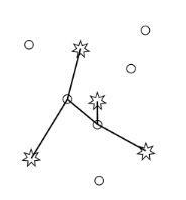
\includegraphics[width = 5cm]{../Codes/DynamicProgramming/SteinerTree.png}
% \addfile{../Codes/DynamicProgramming/Steiner.cpp}
% \vspace{-15pt}

\subsection{Matrix Chain Multiplication}
\addfile{../Codes/DynamicProgramming/MatrixChainMultiplication.cpp}

\subsection{Digit DP} 
\vspace{-5pt}
Counts the amount of numbers in $[l, r]$ such are divisible by $k$. (flag $nonzero$ is for different lengths)  \\
It can be reduced to $dp(i, x, small)$, and has to be solve like $f(r) - f(l - 1)$ \\
\vspace{-5pt}
\addfile{../Codes/DynamicProgramming/Digit.cpp}
\vspace{-15pt}

\subsection{Knapsack 0/1}
\addfile[5-7]{../Codes/DynamicProgramming/Knapsack01.cpp}

\subsection{Convex Hull Trick \complexity{n^2} $\Rightarrow$ \complexity{n}}
$ dp[i] = \min_{j < i}(dp[j] + b[j] * a[i]) $ \\
$ dp[i][j] = \min_{k < j}(dp[i - 1][k] + b[k] * a[j]) $ \\
$ b[j] \geq b[j + 1] \text{ optionally } a[i] \leq a[i + 1] $ \\ 
\addfile[1-41]{../Codes/DynamicProgramming/ConvexHullTrick.cpp}

\subsection{Divide and conquer \complexity{kn^2} $\Rightarrow$ \complexity{k \cdot nlogn} } 
Split the array of size $n$ into $k$ continuous groups. $k \leq n$ \\
$ cost(a, c) + cost(b, d) \leq cost(a, d) + cost(b, c)$ with $a \leq b \leq c \leq d$ \\
\addfile{../Codes/DynamicProgramming/DivideAndConquer.cpp}

\subsection{Knuth optimization \complexity{n^3} $\Rightarrow$ \complexity{n^2} } 
$ dp[l][r] = \min_{l \leq k \leq r}\{dp[l][k] + dp[k][r]\} + cost(l, r)$ \\
\addfile[4]{../Codes/DynamicProgramming/knuth.cpp}

\subsection{Do all submasks of a mask}
\begin{code}
for (int B = A; B > 0; B = (B - 1) & A)
\end{code}


  \nsection{Game Theory}

\subsection{Grundy Numbers}
\ncomment{If the moves are consecutive $S = \{1, 2, 3,..., x\}$ the game can be solved like $stackSize \pmod{x + 1} \neq 0$}
\addfile{../Codes/GameTheory/GrundyNumbers.cpp}
  \nsection{Combinatorics}

\subsection{Catalan}
\addfile{../Codes/Math/Combinatorics/Catalan.cpp}

\subsection{Factorial}
\addfile{../Codes/Math/Combinatorics/Factorial.cpp}

\subsection{Factorial mod small prime}
\addfile{../Codes/Math/Combinatorics/Factorial mod small prime.cpp}

\subsection{Choose}
\begin{gather*}
  \binom{n}{k} = \binom{n - 1}{k - 1} + \binom{n - 1}{k} \\
  \binom{n}{k_1, k_2, ..., k_m} = \frac{n!}{k_1! * k_2! * ... * k_m!}
\end{gather*}
\addfile{../Codes/Math/Combinatorics/Choose.cpp}

\subsection{Pascal}
\addfile{../Codes/Math/Combinatorics/Pascal.cpp}

\subsection{Stars and bars}
Enclosing $n$ objects in $k$ boxes
\begin{gather*}
\binom{n + k - 1}{k - 1} = \binom{n + k - 1}{n}
\end{gather*}
\vspace{-15pt}


\subsection{Lucas}
\ncomment{Changes $\binom{n}{k} \bmod{p}$, with $n \geq 2e6, k \geq 2e6$ and $p \leq 1e7$ }
\begin{gather*}
\binom{n}{k} \equiv \prod_{i = 0}^{n}\binom{n_i}{k_i} \bmod{p}
\end{gather*}
\addfile{../Codes/Math/Combinatorics/Lucas.cpp}

\subsection{Burnside lemma}

Burnside's lemma is a result in group theory that can help when counting objects with symmetry taken into account. It gives a formula to count objects, where two objects that are related by a symmetry (rotation or reflection, for example) are not to be counted as distinct.

let $G$ be a finite group. For each $g$ in $G$ let $f(g)$ denote the set of elements that are fixed by $g$.

\begin{gather*}
  |classes| = \frac{1}{|G|} \cdot \sum_{g \in G} f(g)  
\end{gather*}

\vspace{-5pt}

  \nsection{Number Theory}

\subsection{Goldbach conjecture}
\begin{itemize}[noitemsep]
  \item All number $\geq$ 6 can be written as sum of 3 $primes$
  \item All even number > 2 can be written as sum of 2 $primes$
\end{itemize}

\subsection{Prime numbers distribution}
Amount of primes approximately $\frac{n}{\ln(n)}$

\subsection{Sieve of Eratosthenes}
To factorize divide $x$ by $factor[x]$ until is equal to $1$ \\
\addfile[3]{../Codes/NumberTheory/Factorize sieve.cpp} 
Use it if you need a huge amount of $phi[x]$ up to some N 
\addfile[3]{../Codes/NumberTheory/Phi sieve.cpp} 

\subsection{Phi of euler}
\addfile{../Codes/NumberTheory/Phi.cpp}

\subsection{Miller-Rabin}
\addfile{../Codes/NumberTheory/Miller Rabin.cpp}

\subsection{Pollard-Rho}
\addfile{../Codes/NumberTheory/Pollard Rho.cpp}

\subsection{Amount of divisors}
\addfile{../Codes/NumberTheory/Amount of divisors.cpp}

% 2 3 5 7 11 13 17 19 23 29
% 31 37 41 43 47 53 59 61 67 71
% 73 79 83 89 97 101 103 107 109 113
% 127 131 137 139 149 151 157 163 167 173
% 179 181 191 193 197 199 211 223 227 229
% 233 239 241 251 257 263 269 271 277 281
% 283 293 307 311 313 317 331 337 347 349
% 353 359 367 373 379 383 389 397 401 409
% 419 421 431 433 439 443 449 457 461 463
% 467 479 487 491 499 503 509 521 523 541
% 547 557 563 569 571 577 587 593 599 601
% 607 613 617 619 631 641 643 647 653 659
% 661 673 677 683 691 701 709 719 727 733
% 739 743 751 757 761 769 773 787 797 809
% 811 821 823 827 829 839 853 857 859 863
% 877 881 883 887 907 911 919 929 937 941
% 947 953 967 971 977 983 991 997 1009 1013
% 1019 1021 1031 1033 1039 1049 1051 1061 1063 1069
% 1087 1091 1093 1097 1103 1109 1117 1123 1129 1151
% 1153 1163 1171 1181 1187 1193 1201 1213 1217 1223
% 1229 1231 1237 1249 1259 1277 1279 1283 1289 1291
% 1297 1301 1303 1307 1319 1321 1327 1361 1367 1373
% 1381 1399 1409 1423 1427 1429 1433 1439 1447 1451
% 1453 1459 1471 1481 1483 1487 1489 1493 1499 1511
% 1523 1531 1543 1549 1553 1559 1567 1571 1579 1583
% 1597 1601 1607 1609 1613 1619 1621 1627 1637 1657
% 1663 1667 1669 1693 1697 1699 1709 1721 1723 1733
% 1741 1747 1753 1759 1777 1783 1787 1789 1801 1811
% 1823 1831 1847 1861 1867 1871 1873 1877 1879 1889
% 1901 1907 1913 1931 1933 1949 1951 1973 1979 1987
% 1993 1997 1999 2003 2011 2017 2027 2029 2039 2053
% 2063 2069 2081 2083 2087 2089 2099 2111 2113 2129
% 2131 2137 2141 2143 2153 2161 2179 2203 2207 2213
% 2221 2237 2239 2243 2251 2267 2269 2273 2281 2287
% 2293 2297 2309 2311 2333 2339 2341 2347 2351 2357
% 2371 2377 2381 2383 2389 2393 2399 2411 2417 2423
% 2437 2441 2447 2459 2467 2473 2477 2503 2521 2531
% 2539 2543 2549 2551 2557 2579 2591 2593 2609 2617
% 2621 2633 2647 2657 2659 2663 2671 2677 2683 2687
% 2689 2693 2699 2707 2711 2713 2719 2729 2731 2741
% 2749 2753 2767 2777 2789 2791 2797 2801 2803 2819
% 2833 2837 2843 2851 2857 2861 2879 2887 2897 2903
% 2909 2917 2927 2939 2953 2957 2963 2969 2971 2999
% 3001 3011 3019 3023 3037 3041 3049 3061 3067 3079
% 3083 3089 3109 3119 3121 3137 3163 3167 3169 3181
% 3187 3191 3203 3209 3217 3221 3229 3251 3253 3257
% 3259 3271 3299 3301 3307 3313 3319 3323 3329 3331
% 3343 3347 3359 3361 3371 3373 3389 3391 3407 3413
% 3433 3449 3457 3461 3463 3467 3469 3491 3499 3511
% 3517 3527 3529 3533 3539 3541 3547 3557 3559 3571 

% Big primes near to $10^n$ \\
% 9941 9949 9967 9973 10007 10009 10037 10039 10061 10067 10069 10079
% 99961 99971 99989 99991 100003 100019 100043 100049 100057 100069
% 999959 999961 999979 999983 1000003 1000033 1000037 1000039
% 9999943 9999971 9999973 9999991 10000019 10000079 10000103 10000121
% 99999941 99999959 99999971 99999989 100000007 100000037 100000039 100000049
% 999727999 999997489 999994007 999988243 999992153 999999893 999999929 999999937 1000000007 1000000009 1000000021 1000000033 1070777777
% 1000002193 1000008223 1000009999 1000027163

\subsection{Bézout's identity} 
\ncomment{$a_1 * x_1 + a_2 * x_2 + ... + a_n * x_n = g $}
\ncomment{$g = \gcd(a_1, a_2, ..., a_n)$ }

\subsection{GCD}
\ncomment{$a \leq b; \gcd(a + k, b + k) = \gcd(b - a, a + k)$}
% \addfile{../Codes/NumberTheory/GCD.cpp}
\vspace{-15pt}

\subsection{LCM}
\ncomment{$x = p * lcm(a_1, a_2, ..., a_k) + q, 0 \leq q \le lcm(a_1, a_2, ..., a_k)$}
\ncomment{$x \pmod{a_i} \equiv q \pmod{a_i}$ as $a_i \mid lcm(a_1, a_2, ..., a_k)$ \\}
% \addfile{../Codes/NumberTheory/LCM.cpp}
\vspace{-15pt}

\subsection{Euclid}
\addfile{../Codes/NumberTheory/Euclid.cpp}

\subsection{Chinese remainder theorem}
\addfile{../Codes/NumberTheory/Chinese remainder theorem.cpp}
  \nsection{Math}

\subsection{Bits}
\begin{tabular}{ |p{3cm}|p{5cm}|  }
  \hline  
  \rowcolor{Gray} 
  \multicolumn{2}{|c|}{Bits++} \\
  \rowcolor{Gray} 
  \hline
  Operations on $int$ & Function \\
  \hline
  \texttt{x \& -x} & Least significant bit in $x$ \\
  \rowcolor{Gray} 
  \texttt{\_\_lg(x)} & Most significant bit in $x$ \\
  \texttt{c = x\&-x, r = x+c; (((r\^{}x) >> 2)/c) | r} & Next number after $x$ with same number of bits set \\
  \hline
  \rowcolor{Gray} 
  \_\_builtin\_ & Function \\
  \hline 
  popcount(x) & Amount of 1's in $x$ \\
  \rowcolor{Gray} 
  clz(x) & 0's to the \textbf{left} of biggest bit \\
  ctz(x) & 0's to the \textbf{right} of smallest bit \\
  \hline
\end{tabular}

\subsection{Bitset}
\begin{tabular}{ |p{3cm}|p{5cm}|  }
  % \rowcolors{3}{gray}{white}
  \hline 
  \rowcolor{Gray} 
  \multicolumn{2}{|c|}{Bitset<Size>} \\
  \hline
  \rowcolor{Gray} 
  Operation & Function \\
  \hline
  \_Find\_first() & Least significant bit \\
  \rowcolor{Gray} 
  \_Find\_next(idx) & First set bit after index $idx$ \\
  any(), none(), all() & Just what the expression says \\
  \rowcolor{Gray} 
  set(), reset(), flip() & Just what the expression says x2 \\
  to\_string('.', 'A') & Print 011010 like .AA.A. \\
  \hline
\end{tabular}

\subsection{Probability}
\subsubsection*{Conditional} 
The event A happens and the event B has already happened
\[ P(A | B) = \frac{P(A \cap B)}{P(B)} \] \\
If \textbf{independent} events
\[ P(A|B) = P(A) , P(B|A) = P(B) \]

\subsubsection*{Bayes theorem}
\[ P(A|B) = \frac{ P(B | A) \cdot P(A) }{ P(B) } \]

\subsubsection*{Binomial}
\[ B = {n \choose x} \cdot p^{x} \cdot (1 - p)^{n-x} \]
$n$	=	number of trials \\
$x$	=	number of \textbf{success} from $n$ trials \\
$p$	=	probability of \textbf{success} on a single trial


\subsubsection*{Geometric}
Probability of success at the $nth$-event after failing the others
\[ G = (1 - p)^{n - 1} \cdot p \]
$n$	=	number of trials \\
$p$	=	probability of \emph{success} on a single trial


\subsubsection*{Poisson}
\[ Po = \frac{\lambda ^ k \cdot e ^ {-\lambda}}{k!} \]
$\lambda$ = number of times an event is expected (occurs / time)  \\
$k$ = number of occurring events in the limited period of time \\

Example: The event happens 4 times per minute and we want $k$ events to happen in 10 minutes, then $\lambda = 4 \cdot 10 = 40$

\subsubsection*{Expected value}
\[ E_x = \sum_{\forall x} x \cdot p(x) \]



\subsection{Simplex}
\addfile{../Codes/Math/Simplex.cpp}

\subsection{Xor basis}
\addfile{../Codes/Math/Xor basis.cpp}

  \section{Bit tricks}
\vspace{-5pt}

\subsection{Xor Basis}
Keeps the set of all xors among all possible subsets \\
\addfile{../Codes/Math/Xor Basis.cpp}

\begin{tabular}{ |p{3cm}|p{5cm}|  }
  \hline  
  \rowcolor{Blue} 
  \multicolumn{2}{|c|}{Bits++} \\
  \hline
  \rowcolor{LightBlue2} 
  Operations on $int$ & Function \\
  \hline
  \texttt{x \& -x} & Least significant bit in $x$ \\
  \rowcolor{Gray} 
  \texttt{\_\_lg(x)} & Most significant bit in $x$ \\
  \texttt{c = x\&-x, r = x+c; (((r\^{}x) >> 2)/c) | r} & Next number after $x$ with same number of bits set \\
  \hline

  \rowcolor{LightBlue2} 
  \_\_builtin\_ & Function \\
  \hline 
  popcount(x) & Amount of 1's in $x$ \\
  \rowcolor{Gray} 
  clz(x) & 0's to the \textbf{left} of biggest bit \\
  ctz(x) & 0's to the \textbf{right} of smallest bit \\
  \hline
\end{tabular}

\subsection{Bitset} 
\vspace{-5pt}

\begin{tabular}{ |p{3cm}|p{5cm}|  }
  % \rowcolors{3}{gray}{white}
  \hline 
  \rowcolor{Blue} 
  \multicolumn{2}{|c|}{Bitset<Size>} \\
  \hline
  \rowcolor{LightBlue2} 
  Operation & Function \\
  \hline
  \_Find\_first() & Least significant bit \\
  \rowcolor{Gray} 
  \_Find\_next(idx) & First set bit after index $idx$ \\
  any(), none(), all() & Just what the expression says \\
  \rowcolor{Gray} 
  set(), reset(), flip() & Just what the expression says x2 \\
  to\_string('.', 'A') & Print 011010 like .AA.A. \\
  \hline
\end{tabular}

% 


  \section{Geometry} 
\addfile{../Codes/Geometry/Geometry.cpp}

%%%%%%%%%%%%%%%%%%%%%%%%%%%%%%%%%%%%%%%%%%%%%%%%%%%%%%%%%%%%%%%%
\nsection{Points}

\subsection{Points}
\addfile[1-52]{../Codes/Geometry/Point.cpp}

\subsection{Angle between vectors}
\addfile{../Codes/Geometry/Angle between vectors.cpp}

\subsection{Closest pair of points \complexity{N \cdot log N}}
\addfile{../Codes/Geometry/Closest pair of points.cpp}

\subsection{Projection}
\addfile{../Codes/Geometry/Projection.cpp}

\subsection{KD-Tree}
\ncomment{build: \complexity{N \cdot logN}, nearest: \complexity{logN}}
\addfile[8]{../Codes/Geometry/KD Tree.cpp}

%%%%%%%%%%%%%%%%%%%%%%%%%%%%%%%%%%%%%%%%%%%%%%%%%%%%%%%%%%%%%%%%  

\nsection{Lines and segments}

\subsection{Line}
\addfile{../Codes/Geometry/Line.cpp}

\subsection{Segment}
\addfile{../Codes/Geometry/Segment.cpp}

\subsection{Distance point-line}
\addfile{../Codes/Geometry/Distance point line.cpp}

\subsection{Distance point-segment}
\addfile{../Codes/Geometry/Distance point segment.cpp}

\subsection{Distance segment-segment}
\addfile{../Codes/Geometry/Distance segment segment.cpp}

%%%%%%%%%%%%%%%%%%%%%%%%%%%%%%%%%%%%%%%%%%%%%%%%%%%%%%%%%%%%%%%%

\nsection{Circles}

\subsection{Circle}
\addfile{../Codes/Geometry/Circle.cpp}

\subsection{Distance point-circle}
\addfile{../Codes/Geometry/Distance point circle.cpp}

\subsection{Minimum enclosing circle \complexity{N} wow!!}
\addfile{../Codes/Geometry/Minimum enclosing circle.cpp}

\subsection{Common area circle-polygon \complexity{N}}
\addfile{../Codes/Geometry/Common area circle polygon.cpp}

%%%%%%%%%%%%%%%%%%%%%%%%%%%%%%%%%%%%%%%%%%%%%%%%%%%%%%%%%%%%%%%%

\nsection{Polygons}

\subsection{Area of polygon \complexity{N}}
\addfile{../Codes/Geometry/Area polygon.cpp}

\subsection{Convex-Hull \complexity{N \cdot logN}} 
\addfile{../Codes/Geometry/Convex hull.cpp}

\subsection{Cut polygon by a line \complexity{N}}
\addfile{../Codes/Geometry/Cut polygon line.cpp}

\subsection{Perimeter \complexity{N}}
\addfile{../Codes/Geometry/Perimeter.cpp}

\subsection{Point in polygon \complexity{N}}
\addfile{../Codes/Geometry/Point in polygon.cpp}

\subsection{Point in convex-polygon \complexity{logN}}
\addfile{../Codes/Geometry/Point in convex polygon.cpp}

\subsection{Is convex \complexity{N}}
\addfile{../Codes/Geometry/Is convex.cpp}

%%%%%%%%%%%%%%%%%%%%%%%%%%%%%%%%%%%%%%%%%%%%%%%%%%%%%%%%%%%%%%%%

\nsection{Geometry misc}

\subsection{Radial order}
\addfile{../Codes/Geometry/Radial order.cpp}

\subsection{Sort along a line \complexity{N \cdot logN}}
\addfile{../Codes/Geometry/Sort along line.cpp} 
  // for (int j = i & -i; j != i; j = (j - i)&i) {
  
\end{document}
